\chapter{Cheating}

\section{Definition}
If an aggregator changes the sensor readings reported by its children to skew the final aggregated result is consider as cheating.

\section{Aim}
Aim of this section is to detect the cheater with given definition. 

\section{Assumptions}
We make an assumption that the cheater can not say NACK during verification phase. If a cheater is allowed to send NACK message then it can send NACK messages all the time and create a lot of traffic in the network which might create Denial of service attack. 
\begin{exmp}
	\begin{figure}[t]
		\label{fig:cheating}
		\centering
			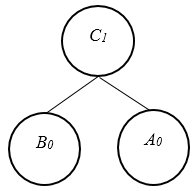
\includegraphics[width=0.2\textwidth]{images/commitment-tree-2.png}
			\caption{cheating}
	\end{figure}	
	Fig \ref{fig:cheating} shows a commitment tree and they have data-items defined as follows.\\
	\textbf{No cheating}\\
	$A_{0} = <A_{id},1,10, H(N||1||10)>$\\
	$B_{0} = <B_{id},1,20, H(N||1||20)>$\\
	$C_{1} = <C_{id},2,30, H(N||2||30||A_{0}||B_{0})>$\\
	\textit{offpath}\\
	$A,B$ receives $C_{1}$ from the base station.
	$A$ receives $B_{0}$ from $C$ and vice versa.\\
	$A_{0} + B_{0}$ = $<2,30,H(N||2||30||A_{0}||B_{0})> = C_{1}$ (by A)\\
	$A_{0} + B_{0}$ = $<2,30,H(N||2||30||A_{0}||B_{0})> = C_{1}$ (by B)\\
	\textbf{Cheating by replacing data-items}\\
		$C$ replaces $A_{0},B_{0}$ with $A'_{0},B'_{0}$\\
		$A'_{0} = <A_{id},1,100, H(N||1||100)>$\\
		$B'_{0} = <B_{id},1,200, H(N||1||200)>$\\
		$C'_{1} = <C_{id},2,300, H(N||2||300||A'_{0}||B'_{0})>$\\
		\textit{verification}\\
		$A_{0}+B'_{0} = <2,210,H(N||2||210||A_{0}||B'_{0})> \neq C'_{1}$(by A)\\
		$A'_{0}+B_{0} = <2,120,H(N||2||120||A'_{0}||B_{0})> \neq C'_{1}$(by B)\\
	\textbf{Cheating by tampering with data-items}\\
		$C$ tampers $A_{0},B_{0}$'s value field\\
		$A'_{0} = <A_{id},1,100, H(N||1||10)>$\\
		$B'_{0} = <B_{id},1,200, H(N||1||20)>$\\
		$C'_{1} = <C_{id},2,300, H(N||2||300||A''_{0}||B_{0})>$\\
		$C''_{1} = <C_{id},2,300, H(N||2||300||A_{0}||B''_{0})>$\\
		\textit{offpath}\\
		$A$ receives $B''_{0} = <B_{id},1,290,H(N||1||20)>$ from $C$\\
		$B$ receives $A''_{0} = <A_{id},1,280,H(N||1||10)>$ from $C$\\
		\textit{verification}\\
		$A_{0}+B''_{0} = <2,300,H(N||2||300||A_{0}||B''_{0})> \neq C'_{1} \neq C''_{1}$(by A)\\
		$A''_{0}+B_{0} = <2,300,H(N||2||300||A''_{0}||B_{0})> \neq C'_{1} \neq C''_{1}$(by B)\\
	\end{exmp}

% \section{What is not cheating ?}
	
% 	In figure 7.1, A is an aggregator if A is a cheater it can skew the final aggregation result irrespective of B's sensor reading. We do not consider this case as a cheating because A is adjusting its sensor reading, it's not changing the B's sensor reading. 
  
% 	For example, if maximum allowed value = 10\\
  
%   case I: $B_{0}(2)$ = 5, $A_{0}(2)$ = 13, $A_{1}(2)$ = 18. In verification, A will be caught due to out of range off path value.\\

%   case II: $B_{0}(2)$ = 5, $A_{0}(2)$ = 10, $A_{1}(2)$ = 15. $B_{0}^{'}(2)$ = 6, $A_{0}^{'}(2)$ = 9. that's not cheating.\\ 

% 	\begin{figure}[t]
% 		\centering
% 			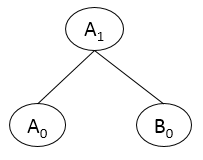
\includegraphics[width=0.2\textwidth]{images/commitment_tree_1.png}\\
% 			\caption{Possible commitment tree}
% 	\end{figure}

% 	Similar arguments can be done for figure 7.2 if A, C  both are cheaters. In that case A is adjusting C's sensor reading to skew the final aggregation result and C will not complain as it is a cheater. We do not consider that as cheating either.

% \begin{figure}[t]
% 	\centering
% 		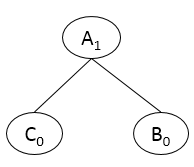
\includegraphics[width=0.2\textwidth]{images/commitment_tree_2.png}
% 		\caption{Possible commitment tree}
% 	\end{figure}

% \section{Probabilistic bound on a cheater}
	
% 	To derive Probabilistic bound on a cheater using following example.

% 	In figure 7.3, all vertices in a commitment tree are unique. And, remember cheater can not say NACK during verification phase. 

% 	\begin{itemize}
		
% 		\item $A_{0}$ says NACK during verification phase it implies that atleast one of the following is \{I\}, \{B, I\}, \{B, M\} is a cheater.
		
% 		\item $A_{0}, B_{0}$ says NACK during verification phase it implies that atleast one of the following is \{I\}, \{M\}, \{C, D, O\} is a cheater.

% 		\item $A_{0}, B_{0}, C_{0}$ says NACK during verification phase it implies that atleast one of the following is \{J ,I\}, \{J, M\}, \{D, O\} is a cheater.

% 		\item $A_{0}, B_{0}, C_{0}, D_{0}$ says NACK during verification phase it implies that atleast one of the following is \{O\}, \{M\}, \{I, J\}, \{E, F, G, H, O\} is a cheater.

% 		\item $A_{0}, B_{0}, C_{0}, D_{0}, E_{0}$ says NACK during verification phase it implies that atleast one of the following is \{O, K\}, \{M, K\}, \{I, J, K\}, \{F, G, H, O\} is a cheater.

% 		\item $A_{0}, B_{0}, C_{0}, D_{0}, E_{0}, F_{0}$ says NACK during verification phase it implies that atleast one of the following is \{I, J, K\}, \{M, N\}, \{O, K\}, \{O, N\} is a cheater.

% 		\item $A_{0}, C_{0}$ says NACK during verification phase it implies that atleast one of the following is \{I\}, \{J\} is a cheater.

% 	\end{itemize}	

% 	\begin{figure}[t]
% 		\centering
% 			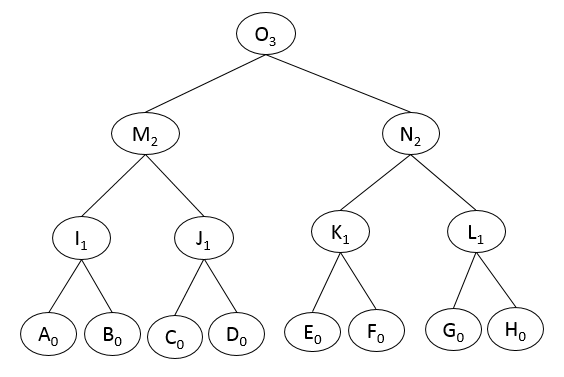
\includegraphics[width=0.7\textwidth]{images/commitment_tree_3.png}
% 			\caption{Possible commitment tree}
% 	\end{figure}

% 	Similar, kind of analysis can be done for figure 7.4 in which all the vertices in the commitment tree are different. 

% 	\begin{figure}[t]
% 		\centering
% 			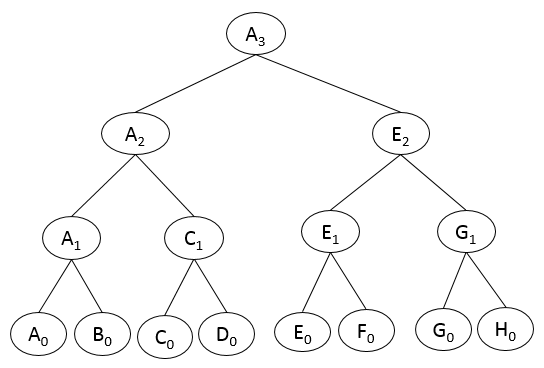
\includegraphics[width=0.7\textwidth]{images/commitment_tree_4.png}
% 			\caption{Possible commitment tree}
% 	\end{figure}

% 	From all above examples we can derive the following pattern as well,

% 	If d = depth of a tree,\\

% 	\begin{tabular}{| l | l |}
%     \hline
%     Depth of a cheater & Minimum number of NACK messages \\ \hline
%     d - 1 & 1 \\ \hline
%     d - 2 & 2 \\ \hline
%     d - 3 & 4 \\ \hline
%     d - 4 & 8 \\ \hline
%   \end{tabular}


% 	\section{ Why do we need digital signatures ?}
% 	Digital signatures allow us to achieve authenticity of the message. 
% 	The labels and signatures have the following format:

% 	id = id

% 	label = $<count, value, commitment>$

% 	signature = $E_{Private_key}( H( N || label ) )$\\
% 	Where \textit{count} is the number of leaf vertices in the subtree rooted at this vertex; 
% 	\textit{value} is the SUM aggregate computed over all the leaves in the subtree; \textit{id} is the sum of all the leaves id in the subtree; \textit{signature} is a cryptographic scheme for demonstrating the authenticity of a message; \textit{N} is the query nonce. 
	
% 	There is one leaf vertex $u_{s}$ for each sensor node s, which we call the leaf vertex of s. The label of $u_{s}$ consists of count = 1, value = $a_{s}$ where $a_{s}$ is the data value of s, and signature is the node's unique ID.

% 	Internal vertices represent aggregattion operations, and have labels that are defined based on their children. Write up examples after talking to Dr.King : Do you have to aggregate ID's as well ?

% 	\section{ Why digital signatures are not sufficient to detect a cheater ? or Why do we need public key infrastructure to detect a cheater ?}
% 	Digital signatures allow us to achieve authenticity of the message but do not provide any mechanism to achieve integrity of the message. To achieve integrity we need public key infrastructure. 

% 	For example, in figure 7.3 one set of possible lables could be the following:

% 	$id_{A} = 1; A_{0} = <1, 5, H(N||1||5)>; Sig A_{0} = E_{K_{A}}(H(N||A_{0})); $

% 	$id_{B} = 2; B_{0} = <1, 6, H(N||1||5)>; Sig B_{0} = E_{K_{B}}(H(N||B_{0})); $

% 	$id_{I} = 3; I_{1} = <2, 11, H(N||2||11||A_{0}||B_{0})>; Sig I_{1} = E_{K_{I}}(H(N||I_{1})); $

% 	$id_{J} = 4; J_{1} = <2, 15, H(N||2||15||C_{0}||D_{0})>; Sig J_{1} = E_{K_{J}}(H(N||J_{1})); $

% 	$id_{M} = 5; M_{2} = <4, 26, H(N||4||26||I_{1}||J_{1})>; Sig M_{2} = E_{K_{M}}(H(N||M_{2})); $

% 	Above labels and signatures are the case where no one is cheating in the network. If A, B say NACK message during the verification phase it means either M or I is a cheater. To preceisely find who is cheater we have following problems:

% 	\begin{itemize}
% 		\item M can say it received ($I_{1}^{'}, Sig I_{1}$) eventhough it received ($I_{1}, Sig I_{1}$) from I.
% 		\item M can not verify that it received ($I_{1}^{'}, Sig I_{1}$) instead of ($I_{1}, Sig I_{1}$) from I.
% 	\end{itemize}
% 	Because of this we can not not detect cheater between I, M. The fundamental problem is that signatures can be verified only by the base station and not by any of the intermediate nodes. We want the ability in which an intermediate node can verify the signatures from its children. And that is why we need public key infrastructure.
